\documentclass[aip,amsmath, reprint, author-year]{revtex4-1}
\usepackage{url}
\usepackage[utf8]{inputenc}
\usepackage{hyperref}
\usepackage{graphicx} % for graphics
%\usepackage{listings} % for code listtings
%\usepackage{color}

%\setcitestyle{round, author-year}

\setcounter{page}{1}

%\bibliographystyle{aipauth4-1.bst}

\begin{document}

\begin{abstract}
An approach to generate generalised process capability data in order to populate and add functionality to a process capability database.
A description of the concept of generalisation, uses and implementation.
\end{abstract}

\title{Concept of using General Process Capability Data - DRAFT}
\author{Andreas Bruun Okholm, s082562\\
Mathias Rask Møller, s082536 }
\affiliation{Technical University of Denmark}
 
\date{\today}
\maketitle

%Introduction

A process capability database (PCDB) is a tool for mechanical designers to get information of what is possible to achieve in production. This is done by storing and displaying statistical information about features on produced components.  
By applying process capability (PC) information in the design process it is possible to reduce: rework, cost, failure rate, assembly problems and increases product performance \citep{tata1999process}.

As mentioned in \citep{tata1999process, tata1999effective, raskokholm} and a number for key challenges has to be addressed to expand the use of PCDB.
\begin{itemize}
	\item Data Communication: The databases are typically not easily searchable which makes it very difficult to find the correct data and in many cases the data sought after data does not exists. Further more the data is not presented in a way which is easily understandable by mechanical designers.
	\item Fragmented Organisation: Development department are dependent on data from production. 
	\item Information Technology: Make a database which is fast, live, global, self populating, up to date and live up to the industry criteria of security and anonymity.
\end{itemize}

There has been a couple of attempts in academia to solve some of these difficulties \citep{thornton2000use, kern2003forecasting, thornton2004variation}, but there hasn't much attention on the subject since indicating there is still issues to resolve before it can be efficiently used in the industry.

In this article we present a concept of data indexing, processing and presentation which tries to make it faster and easier for the mechanical designer to efficiently use process capability data in new designs. 
The general principle is to provide an interface where the data is presented in a much more generalised than typically done in PCDB interfaces. 
The core indexing scheme is simplified, but details are retained or improved using a flexible tagging system. 
Instead of presenting the designer with statistical information, recommended specifications limits based on actual PC is shown directly. 
The specification limits is normalised in regard to the specified dimension making more use out of each dataset, minimising the risk of PC requests not returning any results. 

Combined with advances in information technology we hope this will help make PCDBs a viable tool in the mechanical design process. 

\section{Indexing}

\begingroup
\squeezetable

\begin{table*}
\begin{ruledtabular}
\caption{\label{tab:sampleset} Measurement set - As stored in the PCDB}
\begin{tabular}{lllllllll}
\textbf{Material*} 		& \textbf{Process*} 		& \textbf{Meas. Equipment}  	& \textbf{Target*} 	& \textbf{LSL} 	& \textbf{USL} 	& \textbf{Mean Shift*} 	& \textbf{Std.}   $\hat{\sigma}$ * & 	\\
Thermoplastic 			& Moulding			& CT Scanning				& 3.00			& 2.99		& 3.01		& -0.0486			& 0.0032				\\
 - ABS, PC blend		& - Injection Mould.		& Zeiss metrotom 800	\\
\\
\textbf{General Tag (1)} 	& \textbf{General Tag (2)} & \textbf{General Tag (3)} 	& \textbf{Geometry}		& \textbf{Measurement Date} 	& \textbf{N samples} 	\\
Mould Type			& Product color			& Production run			& Diameter				& 13 oct. 2013  			& 12\\
- Steel 				& - Red				& - PR3				\\
- - NAK80 
\end{tabular}%
\end{ruledtabular}
\end{table*}
\endgroup


PCDBs needs to be indexed to efficiently retrieve data of relevance to the current design. 
The data stored in a PCDB is typically measurement sets; the statistical result of a number of measurements from a given part dimension combined with the design characteristics (DC). 
Feature, geometry, material and process is suggested by \cite{kern2003forecasting} to be the primary DCs. 
For each primary DC there exists a tree structure of possibilities. An example of an index using Kerns proposed design index could be "Plane", "Position", "Aluminium", "Turning" as feature, geometry, material and process respectively. 

We propose to use \emph{material} and \emph{process} as the only required DCs. 
\emph{Geometry} information: distance, radius, diameter or positions is readily available from the measurement tool and should be stored as well, but not necessarily used when querying the database.
This is combined with a \emph{tagging system}, where additional tags can be inputted. 
Common tags can be selected from tree structure. 
Tags gives flexibility since more than one tag can be applied to one measurement set and it is possible to index for DCs that are specific to a single production method or material. 

Example: For injection moulding it would be interesting to index the following DCs:
\begin{itemize}
\item Material type of the mould: aluminium, steel, hardened, etc.
\item Mould/Process iterations (T0, T1, T2, ...) could also give valuable insights of which specification limits requires mould rework or process adjustment. 
\item Tagging dimensions measured a crosses parting lines could potentially showing a general increase in desired specification limits.
\end{itemize}
It would not be possible to index these DCs, which are specific for the process without having optional tags. 
A complete database record of a sample set can be seen in table \ref{tab:sampleset} showing all data connected to the sampleset. 

\emph{No feature index:}
In casting and injection moulding, two of the most used processes for mass produced part, feature is not necessarily an important DC. 
The individual features are manufactured by the same computer-aided manufacturing (CAM) milling machine with the same process parameters. 
For features with properties such as high length to width ratios could be optionally tagged. 
In a fully integrated robust design process interaction between components are reduced to as small and simple surfaces as possible further reducing the need for a features index.

\section{Processing Capability Data}

Processing the capability data consists of three steps: 

\begin{enumerate}
	\item Compute the process capability specification limit (PCSL) - the required specification limits (tolerance) to achieve a desired performance using the given process capability.
	\item Normalise the PCSLs so it is independent of dimension.
	\item Fit operating curves to the PCSL data grouped by different design characteristics.
\end{enumerate}

\subsection{Process Capability Specification Limit}
The process capability indices ($C_p$ and $C_{pk}$) described by \cite{kane1986process} has been widely adopted in statistical process control, been extended and further researched for better understanding \citep{wu2009overview}. 
Instead of looking at process mean $\mu$, standard deviation $\sigma$ and specification upper and lower limits $USL$, $LSL$ using process capabilities indices (PCIs) transforms these values into unit less numbers, which provides a quick overview of how a process is performing.

The PCIs ability to transform process variables of any object into unit less capability index can be reversed to calculate desirable specification limits. For en example the commonly used PCI $C_{pk}$ 
\begin{equation}
	C_{pk} = \frac{d - | \mu - m|}{3 \sigma} \nonumber
\end{equation}
can be reversed
\begin{equation}
	d = 3 C_{pk} \sigma + | \mu - m|
\end{equation}
Where $d = (USL - LSL) / 2$ is half the specification limit and $m = (USL + LSL) / 2$ is the midpoint between the specification limits. When $d$ is reversely used to estimated the required tolerance to achieve the desired process capability index value we call this the process capability specification limit (PCSL). 

Using the data from table \ref{tab:sampleset} and a $C_{pk} = 1.66$. The PCSL is computed: 
\begin{align*}
PCSL &= 3 \cdot 1.66 \cdot 0.0032 \, \mathrm{mm}
+ |0.0486  \, \mathrm{mm}| \\
&= 0.0645  \, \mathrm{mm}
\end{align*}


There are several commonly used PCIs each serving their purpose \citep{wu2009overview, taguchi1986introduction}
\begin{itemize}
	\item $C_a$ : Closeness of process mean to target 
	\item $C_p$ : Relative size of variation
	\item $C_{pk}$ : Amount of nonconforming (\%NC)
	\item $C_{pm}$ : Value loss (Taguchi loss function)
	\item $C_{pmk}$: Version of $C_{pm}$,  sensitive to mean shift. 
\end{itemize}

Visualising the $CPIs = 1$  shows how a process on target $C_a = 1$ allows the same variation for all PCIs see figure \ref{fig:CPI}. The line for $C_{pm}$ is in below that of $C_{pk}$ except for values of $C_a$ close to 1. 
Using $C_{pm}$ will in general be more conservative resulting in larger specification limits than $C_{pk}$. The plot shown is for a capability equal to one for higher values this effect is even more pronounced.

\begin{figure}
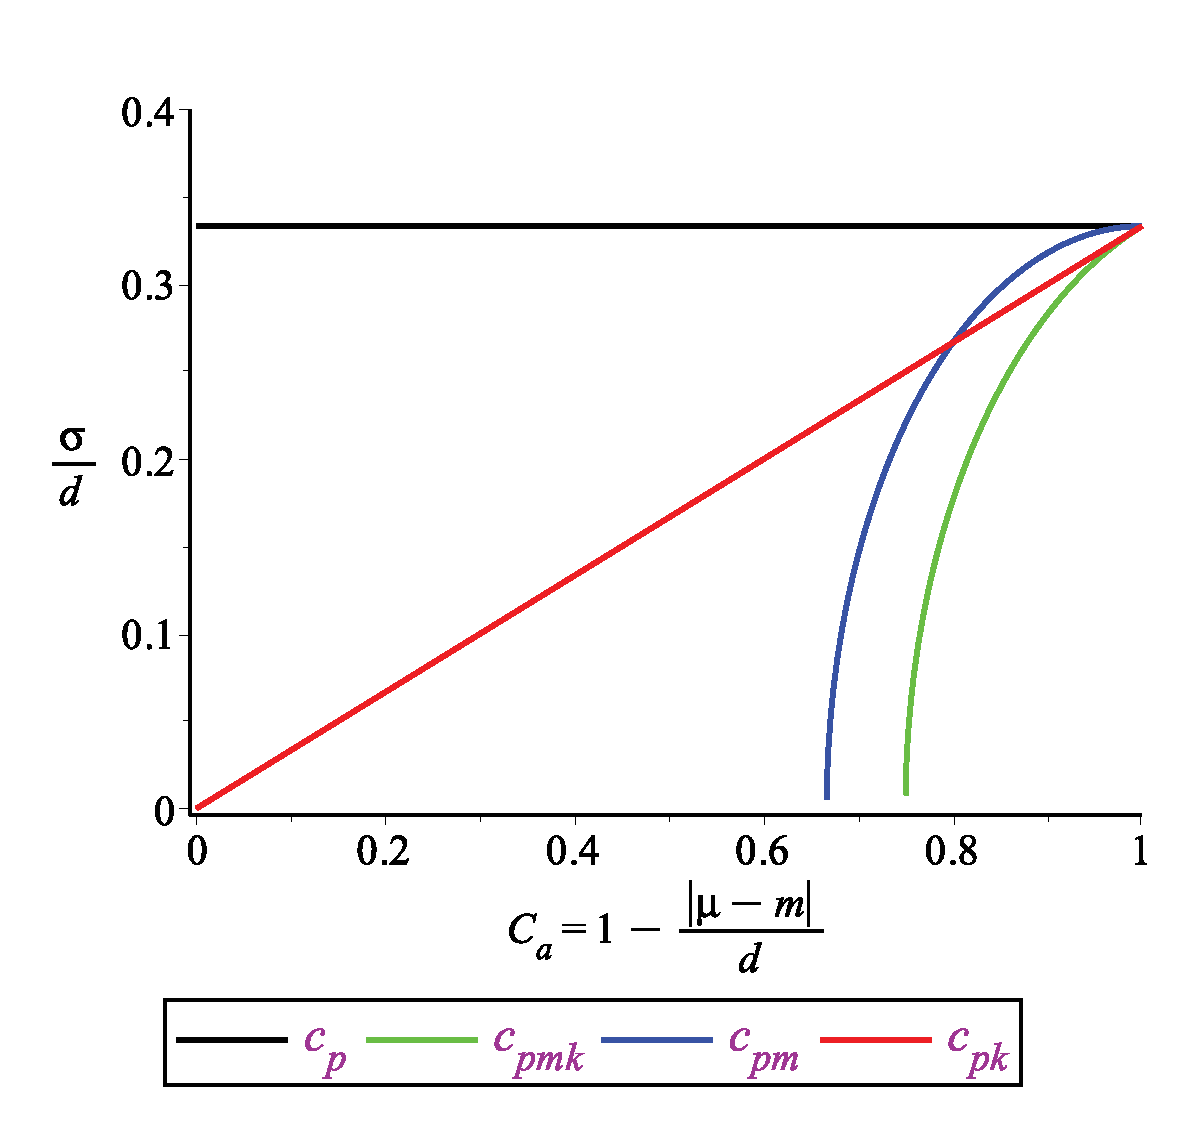
\includegraphics[width=0.45\textwidth]{graph_postscript_test.eps}
\caption{\label{fig:CPI} Nomalised standard deviation as a function of normalised meanshift. $C_p$ referens only to the variance of the process. $C_{pk}$ is related to the yield of the product. $C_{pm}$ takes a loss function in to account relates to a target dimension. $C_{pmk}$ takes both the yield of the product and a loss function. }
\end{figure}

For the purpose of our database we have chosen to use $C_{pk}$, since it provides the most easily understandable result - directly related to the yield of the process. The yield of a process is within
\begin{equation}
	2\Phi(3C_{pk})-1 \leq \text{yield} < \Phi(3C_{pk}) \nonumber
\end{equation}

where $\Phi(\cdot)$ is the cumulative distribution function of the standard normal distribution N(0,1) \citep{boyles1991taguchi}. For typical capability levels the resulting non-conforming products in parts per million (ppm) is listed in table \ref{tab:cpl_nc}

\begin{table}
\begin{ruledtabular}
\caption{\label{tab:cpl_nc} $C_{pk}$ Non-conformities}
\begin{tabular}{llll}
  $\mathbf{C}_{pk}$	& $\sigma$ level	& $\mathbf{NC_\mathrm{max}} \mathrm{\ (ppm)}$	&  $\mathbf{NC_\mathrm{min}} \mathrm{\ (ppm)}$	\\
  1.00	& 3		& 2699.8		& 1349.9		\\
  1.33 	& 4 		& 63.3		& 31.7 		\\
  1.50 	& 4.5 	& 6.7		& 3.4		\\
  1.66	& 5		& 0.6		& 0.3		\\
  2.00	& 6		& 0.002		& 0.001		\\
\end{tabular}%
\end{ruledtabular}
\end{table}

The optimal process capability index value depends on the application, however there exists a practice in quality control called six sigma $(6 \sigma)$, which advocates the use of six sigma ($C_{pk} = 2$) for short term process capability will generally improve manufacturing quality and profits \cite{koch2004design}. 

It's assumed that the process drifts over time up to $1.5 \sigma$  (effectively resulting in a sigma level of 4.5), which still results in an acceptable 3.4 ppm defects.
For the PCSL to reflect six sigma production capability the $C_{pk}$ input with each measurement set should be varied from 2.0 to 1.5 $C_{pk}$ depending wether the measurement set reflects the short or long term capability. 
For simplicity we propose to use a value general value of $C_{pk} = 1.66$ to account for a  mixture of long term and short term measurements. 

We have focused on $C_{pk}$ through most of this section.
In situations where the desired tolerances directly influence product performance, for instance in lens optics construction, using the more abstract $C_{pm}$ might make more sense. 


\subsection{Normalization}
The calculated Process Capability Specification Limits (PCSL) are normalised so it can be used to predict PCSLs for any dimension within the limit of the normalisation algorithm. 
This reduces the required amount of data in the database before it's useful for mechanical design since it is possible to use PC information from components of different sizes.

There exists industrial standards used for manufacturing which describe the "normal" relationships between linear dimensions and tolerances. We have analysed the most commonly used standards for general tolerances: American \citeauthor{american1978preferred}, European \citeauthor{ISO286} and the German \citeauthor{DIN7168}. The ANSI and the ISO standards uses the same formula and are quite close to the german DIN standard. 
These standards display a non-linear relationship between tolerance and dimension. For the same level for precision, the tolerances of large dimensions are smaller relatively than for small dimensions. See figure \ref{fig:tolstd}.

The German \citeauthor{DIN16901} and the French \citeauthor{NFT58000} are standards specifically for moulded plastic parts. These standards present an almost linear relationship between tolerance and dimension. This might be due that a major contributing error in moulded parts is a result of creep, since creep errors in general has a linear relationship between overall dimension and error.

\begin{figure}
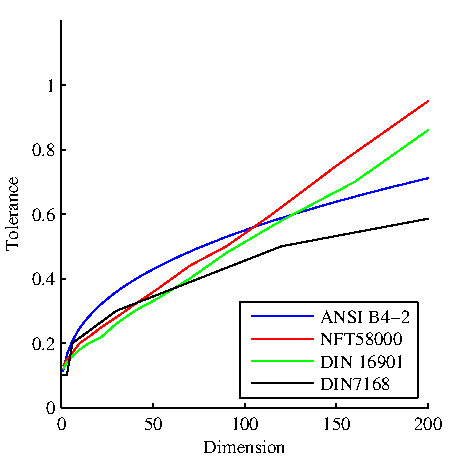
\includegraphics[width=0.5\textwidth]{Tolerance_standards.pdf}
\caption{\label{fig:tolstd} \citeauthor{DIN16901} (POM 120) and \citeauthor{NFT58000} (normal) are standards specifically for moulded plastic components. They are almost linear for sizes above 10 mm. 
\citeauthor{american1978preferred} (gr. 13) and \citeauthor{DIN7168} (medium) describes a general relationship between linear tolerances and dimension. All standards included several levels of precission.}
\end{figure}

These standards are all described using a tables showing the tolerances for a given dimension intervals and precision. 
In a note for \citeauthor{american1978preferred} and later mentioned in \citeauthor{ISO286} a continuous function is described for IT-grades (precision levels) between IT6 to IT16 for dimensions from 2 mm to 500 mm. This function is for unknown reasons not included in newer versions of ISO 286 yet table values seems still estimated using this function.

\begin{align}
	T =& 10^{0.2 (ITG -1)} \cdot i \\
	i =& 0.45 \sqrt[3]{D} + 10^{-3} \, D 
\end{align}

Where $i$ is standard tolerance factor, $D$ is the nominal mean dimension $D = \sqrt{D_{\textrm{min}} D_\textrm{max}}$ in $[mm]$ and $T $ is the tolerance width in $[\mu m]$ , which is equal to $2d$. 

In the generalised PCDB the measurement sets PCSL are normalised using said function because ISO 286 is general practice in the industry. 
Further work on improving the normalisation feature requires more data than what is available to us. Normalization actual data for the different processes.

The IT-grade for the measurement set presented in table \ref{tab:sampleset} can be computed.

\begin{align*}
&\mathrm{ITG} = 5 \cdot \log_{10} \left\{ \frac{T \cdot 10^3}{ 0.45  D^{\frac{1}{3}} + D \cdot10^{-3} }\right\} +1 \\
&\mathrm{ITG_{spec} }= 13.4 \\
&\mathrm{ITG_{actual}} = 12.5
\end{align*}

The $\mathrm{ITG_{actual}}$ is based on the measurements  and is calculated using $T = 2 \, PCSL$ and the $\mathrm{ITG_{spec}}$ is specified by the design and is calculated using $T = 2 \,USL$ for symmetric tolerances. 

\subsection{Analyze normalized data}
A further analysis of the underlying measurements sets is done to present the user with a easier to use data view. Relevant measurements sets are aggregated based on DC's selected by the user. 

To help the user determine which tolerance to use, a accumulated frequency plot of the normalised PCSL is proposed. 
This gives an overview of the current process capability assuming it has not changed since the data has been recorded. 
The plot shows the probability, if production capability were randomly selected, to produced the selected part at a specified $C_{pk}$ and tolerance, see figure \ref{fig:acumfreq}. 
A normal distribution is fitted to the data to show a continuous function.

Selecting a tolerance associated with a low probability will generally impact the price of production since it either: Increases risks of rework to hit the target $C_{pk}$ or requires more precise machines than what is used for the measured components.

\begin{figure}
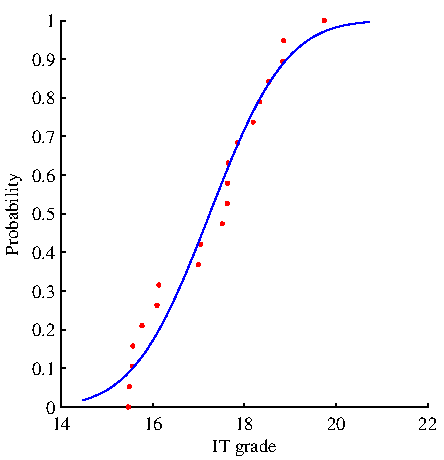
\includegraphics{Acum_freqIT.pdf}
\caption{\label{fig:acumfreq} Accumulated frequency IT grade distribution, $C_{pk} =1.66$. 
20 measurement sets each containing between 3 and 219 samples. Actual data from \cite{thornton2000use}. }
\end{figure}

It is possible to easily compare multiple CDs by displaying them in the same view. In figure \ref{fig:acumfreqF3} PC data from two machines is shown respectively. It is possible to see that the machine marked '1031' performs better than '1032', but '1032' is more consistent.

\begin{figure}
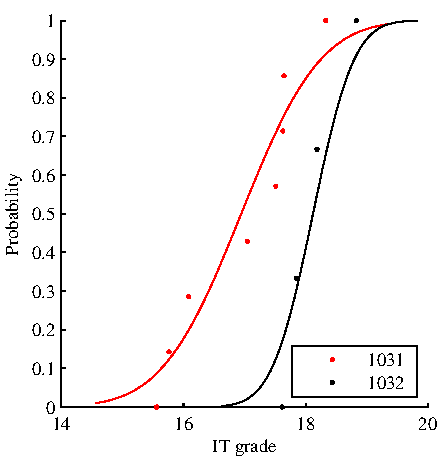
\includegraphics{Acum_freqF3.pdf}
\caption{\label{fig:acumfreqF3} Comparing two differnet DC's. Measurement sets from machine nr. 1031 and 1032 respecfully. Accumulated frequency IT grade distribution, $C_{pk} =1.66$. Actual data from \cite{thornton2000use}. }
\end{figure}

Further consideration are done in order display the information in a more comprehensible way.
\begin{itemize}
\item The tolerance can be shown in $[mm]$ instead of IT-grade for a user selected dimension.
\item In a web environment a popup activated by hover interactivity allow the user to see specifics of each data point.
\item Confidence limits for the estimated distribution should be shown to ensure statistically validity.
\end{itemize}

\section{Statistical Validity}
The user needs to trust the information provided by the PCDB. The uncertainty of the resulting distribution of IT grades is influenced by several factors.
\begin{itemize}
\item More samples in each measurement set will increase certainty. 
\item More measurements sets increases the certainty. 
\item Lower standard deviation of the IT grade distribution will increase the certainty.
\item Higher mean deviations from target $C_a$ will slightly increase the certainty especially at low sample sizes.
\end{itemize}
Sample size and number of measurement sets are the only two possible actionable variables. 

\subsection{Monte Carlo simulaiton}
To model the uncertainty of the IT-grade distribution we have chosen to use Monte Carlo simulation, since it would be very difficult to accurately model analytically. 
We assume that the IT-grade (ITG) from each measurement set is continuous random variate with mean $\mu_{\mathrm{ITG}}$ and standard deviation $\sigma_{\mathrm{ITG}}$ giving $\mathrm{ITG} \sim \mathcal{N} (\mu_{\mathrm{ITG}}, \sigma_{\mathrm{ITG}}^2)$

The randomly generated ITG is converted into a normal distribution of individual measurements X using a fixed target dimension of $m = 100 \mathrm{\ [mm]}$ and closeness to target $C_a = 0.6$. 
The standard deviation $\sigma_{X}$ and mean shift $| \mu - m|$ can be calculated yielding the distribution parameters $\mathrm{X} \sim \mathcal{N} (| \mu - m|, {\mu_{\mathrm{X}}}^2)$. 

Each measurement is generated from the measurement set distribution.
When all the sample data has been generated the process is reversed and the distribution parameters of ITG is estimated. The simulation is run $N$ times.   

We have chosen to estimate the confidence intervals at 50\% and 90\% cumulative probability ($\mathrm{ITG_{50}}, \mathrm{ITG_{90}}$) using the percentile method. The percentile method interval is the interval between the $100 \cdot \alpha$ and $100 \cdot (1-\alpha)$ percentiles of the Monte Carlo distribution of $\mathrm{ITG_{50}}, \mathrm{ITG_{90}}$.

To verify the simulation we compared the confidence interval at $\mathrm{ITG_{50}}$ with a simple approximation of the interval based on the Wilson score interval for the ITG distribution. The Monte Carlo interval width is about $4/5$ of the wilson score, indicating that the Monte Carlo works and that the Wilson score is a fine approximation. 

\begin{figure}
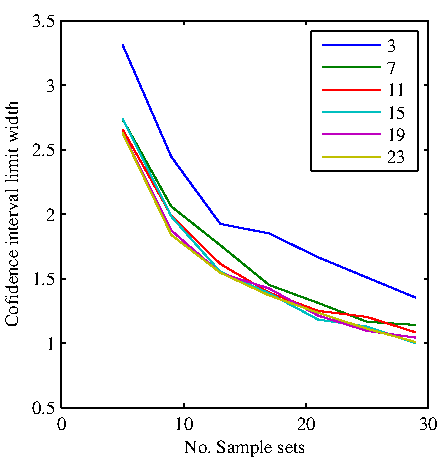
\includegraphics{CLW90_lines.pdf}
\caption{\label{fig:cl_line} Monte Carlo simulation of the cofidence interval width as a function of both sample size and number of measurement sets. Confidence interval width is measured in IT-grades. The number of sample sets has much bigger influence than sample size for sizes above 12 samples.}
\end{figure}


\textbf{Result} Figure \ref{fig:cl_surf} and \ref{fig:cl_line} show the confidence interval width at a cumulative probability of 90 \% ($\mathrm{ITG_{90}}$) as a function of sample size and number of measurement sets . Increasing sample size only have an effect up to about 11 samples, additional measurements does not increase the number of measurement sets. The amount of measurements sets is the main factor for reducing the confidence intervals. If the purpose is too differentiate between DCs then the number of measurements sets is going to limit how small the differences between DCs can be resolved with statistical certainty.


\section{Discussion}


The effect of a low sample size is shown in figure \ref{fig:effect}. the standard deviation of the deviation is overestimated compared the input distribution.

\section*{References}
\bibliography{../PCDBmasterBibliography/PCDB_Master_bib.bib}

\end{document}